\chapter{Case Study}\label{chap:case-study}

In this chapter, we lay out the steps taken and the issues faced during the conversion from Angular components to Web Components. This chapter consists of five sections. The first section provides some information on the build process we are using. The second section describes issues faced that were not specific to Angular or Angular Elements, while the third section contains just Angular-specific issues. The fourth section lists the various optimizations we applied, and the fifth section describes the JS framework wrappers. Note that because of the split between Angular and Web Components issues, the issues are no longer listed out in chronological order. For a chronological overview of the various issues and their relative complexities, see Table~\ref{tab:case-study:chronological-issues}. After the issue sections, we discuss the various JS framework wrappers and how they were created. Lastly, we list optimizations performed along with their effectiveness.

\begin{table}[htbp]
  \begin{tabularx}{\textwidth}{|l|X|l|}
    \toprule
    \textbf{Section}                            & \textbf{Section Name}              & \textbf{Relative Complexity} \\ \midrule
    \ref{sec:case-study:global-css}             & Global CSS                         & simple                       \\ \hline
    \ref{sec:case-study:compatibility}          & Compatibility                      & simple                       \\ \hline
    \ref{sec:case-study:tagname-renaming}       & Tagname renaming                   & simple                       \\ \hline
    \ref{sec:case-study:theming}                & Theming                            & simple                       \\ \hline
    \ref{sec:case-study:non-string-attributes}  & Non-string Attributes              & medium                       \\ \hline
    \ref{sec:case-study:complex-attributes}     & Complex Attributes                 & complex                      \\ \hline
    \ref{sec:case-study:ng-deep}                & ng-deep                            & simple                       \\ \hline
    \ref{sec:case-study:create-custom-element}  & createCustomElement                & simple                       \\ \hline
    \ref{sec:case-study:eventemitters}          & EventEmitters                      & simple                       \\ \hline
    \ref{sec:case-study:hierarchical-injectors} & Hierarchical Injectors             & hard                         \\ \hline
    \ref{sec:case-study:ng-on-init}             & ngOnInit                           & medium                       \\ \hline
    \ref{sec:case-study:casing}                 & Casing in attribute names          & simple                       \\ \hline
    \ref{sec:case-study:directives}             & Angular directives                 & simple                       \\ \hline
    \ref{sec:case-study:ng-content}             & <ng-content>                       & simple                       \\ \hline
    \ref{sec:case-study:attribute-order}        & Angular Attribute Order            & medium                       \\ \hline
    \ref{sec:case-study:bundling-imports}       & Bundling Angular Imports           & hard                         \\ \hline
    \ref{sec:case-study:ivy}                    & Angular Ivy                        & hard                         \\ \hline
    \ref{sec:case-study:searching-for-css}      & Reduce time searching for CSS      & simple                       \\ \hline
    \ref{sec:case-study:css-initial-load}       & Move CSS searching to initial load & simple                       \\
  \end{tabularx}
  \caption{Sections in chronological order along with their relative complexities}
  \label{tab:case-study:chronological-issues}
\end{table}

\section{Build Process}\label{sec:build-process}
The build process that eventually generates the Web Component library consists of a number of stages. These are the following stages:

\begin{itemize}
  \item \emph{Pre-build scripts:} Code runs that manipulates the source code and prepares it for the next process. An example of this is the pre-build script that copies the source code to a \code{build/} folder. This step allows us to transform the source code that is going to be used in the next stage without touching the original files. If we were to change the original files in place, we would also have to undo the replacements. This could prove problematic if a build fails, after which source control is the only way to recover the files.
  \item \emph{Building:} We build the Angular project. In this step, the code in the previously created \code{build/} directory is built into an Angular bundle. When this bundle is loaded on a page, the Web Component library is initialized, and the various Web Components are ready for use.
  \item \emph{Bundling:} Build artifacts generated in the previous step are spread out over several files. Since we want to provide developers with a single bundle that contains all of the required code, we bundle these various files up into a single file.
  \item \emph{Generating of wrappers:} The various wrappers for JS frameworks are generated. This process is described further in Section~\ref{sec:js-framework-wrappers}.
\end{itemize}

\section{Web Component Issues}~\label{sec:web-component-issues}
In this section, we document issues faced that were related to Web Components, as well as our solutions to them. These are issues that are not at all related to the Angular framework and are likely to be faced in other similar projects.

\subsection{WC1: Global CSS}\label{sec:case-study:global-css}
\problemSolution{
  Angular components have a property called \code{encapsulation}\footurl{https://angular.io/guide/view-encapsulation\#view-encapsulation}. This property determines how CSS styles are applied to the component. It has three possible values:

  \begin{itemize}
    \item \emph{ShadowDom:} Global styles are not applied to the component. Only the component's own styles are applied to it.
    \item \emph{Emulated (default):} Global styles are applied to the component as well as its own styles. Other components' styles are not applied to it.
    \item \emph{None:} Global styles, a component's own styles, and other components' styles are applied to this component.
  \end{itemize}

  In the 30MHz codebase, the default (or Emulated) value is used, meaning that both global and component-specific styles are applied to it. This is done by putting both of them in a global stylesheet. This stylesheet then has component-specific selectors added to it, making sure that styles are always scoped to a specific component. An example of this process can be seen in Listing~\ref{lst:case-study:component-css-source} and Listing~\ref{lst:case-study:component-css-compiled}.

  When migrating the Angular components to Web Components, we ensure the components' contents are rendered within a ShadowRoot~\footurl{https://developer.mozilla.org/en-US/docs/Web/API/ShadowRoot}. A ShadowRoot is a separate root within an HTML document that contains its very own document. This document is entirely separated from the parent document, meaning it is not influenced by global styles in that document. This effectively separates the component from the rest of the DOM, thereby also removing the ability of the global 30MHz stylesheet to be applied to it.

}{
  When a component is rendered, we find the global stylesheet on the page. We then copy it into a Constructable Stylesheet~\footurl{https://developers.google.com/web/updates/2019/02/constructable-stylesheets} if it has not already been copied. Constructable Stylesheets are a method of creating CSS stylesheets in JavaScript. These stylesheets can then be used together with the \code{adoptedStylesheets}~\footurl{https://developers.google.com/web/updates/2019/02/constructable-stylesheets\#using_constructed_stylesheets} JavaScript property of a ShadowRoot. Any Constructable Stylesheet placed in the \code{adoptedStylesheets} array is applied to the ShadowRoot similar to how any \code{<style>} tag in a document is applied to that document. The advantage to using this method is that Constructable Stylesheets are simply references that can be re-used by the browser, contrary to regular \code{<style>} or \code{<link rel="stylesheet">} tags, which are parsed from scratch every time the browser encounters them. This means that every time a new instance of a component is created, instead of copying a \code{<style>} or \code{<link rel="stylesheet">} tag and having the browser parse it from scratch (which takes approximately 16ms), we instead add the stylesheet to the \code{adoptedStylesheets} property of the ShadowRoot and have an already-parsed stylesheet applied to the ShadowRoot. We use this method to apply the global 30MHz stylesheet in the component's own ShadowRoot as well by copying that stylesheet to every component's ShadowRoot. Normally this would incur a heavy performance impact, but because of the use of \code{adoptedStylesheets}, the performance impact is minimal.

}

\begin{lstlisting}[language={JavaScript},caption={An example of uncompiled source code for a component},label={lst:case-study:component-css-source}]
// my-component.html
<my-component></my-component>

// my-component.css
:host {
  color: red;
}
\end{lstlisting}

\begin{lstlisting}[language={JavaScript},caption={An example of compiled code for the component in Listing~\ref{lst:case-study:component-css-source}.},label={lst:case-study:component-css-compiled}]
// my-component.html
<my-component _ngcontent-uix-c290></my-component>

// my-component.css
[_ngcontent-uix-c290] {
  color: red;
}
\end{lstlisting}

\subsection{WC2: Compatibility}\label{sec:case-study:compatibility}
\problemSolution{
  While browser support for Web Components is relatively widespread as of this case study~\footurl{https://caniuse.com/?search=components}, it is not yet universal. Additionally, Safari has chosen not to implement support for \emph{Customized Built-In Elements}\footurl{https://www.chromestatus.com/feature/4670146924773376}. This feature allows for extending built-in HTML elements, allowing developers to extend already-existing elements such as the \code{HTMLInputElement} and others. Since the 30MHz dashboard makes use of components that extend native elements (in the form of directives\footurl{https://angular.io/guide/attribute-directives}), we need this feature to make the CC UI library work.
}{
  We add polyfills to the final JS bundle. These are files that add support for unsupported features by implementing them in JavaScript. If the feature a polyfill intends to provide is already supported by the browser, it will fall back to the built-in version. This ensures that they pose little to no performance impact if a given feature is already supported. In particular we use the \ver{custom-elements}\footurl{https://www.npmjs.com/package/@ungap/custom-elements} and \ver{custom-elements-builtin}\footurl{https://www.npmjs.com/package/@ungap/custom-elements-builtin} polyfills. These add support for Web Components (aka Custom Elements) to browsers that do not have it. Additionally, they add support for the previously mentioned \emph{Customized Built-In Elements} feature.
}

\subsection{WC3: Tagname renaming}\label{sec:case-study:tagname-renaming}
\problemSolution{
  As per the Web Components specification, all Web Components are required to have a hyphen in their tag name~\footurl{https://html.spec.whatwg.org/multipage/custom-elements.html\#custom-elements-core-concepts}. Angular components, on the other hand, do not have this requirement. Because of this, there are some components in the 30MHz codebase without a hyphen in their name. In order to export them as Web Components, we need to come up with a tag name with a hyphen in it. In this case we decided to prefix every component with \code{cow-} (for example \code{<cow-checkbox>}). This renaming, however, leads to an issue with components that are being used inside other components. For example say the \code{TripleCheckbox} component renders three checkboxes. Example source code for such a component can be seen in Listing~\ref{lst:case-study:double-checkbox}. If such a component is rendered as a Web Component, it will attempt to render the \code{<checkbox>} HTML tag, not knowing that it has been renamed to \code{<cow-checkbox>}. The result is an empty component.
}{
  We run a pre-build script that replaces the names of components that will be used in the UI library with their prefixed variant. This pre-build script is run in the first stage of our build process, as described in Section~\ref{sec:build-process}. We make sure not to replace native HTML elements by matching the found HTML tags against a list of known native HTML elements.
}

\begin{lstlisting}[language={HTML},caption={Example source code for a \code{TripleCheckbox} component.},label={lst:case-study:double-checkbox}]
<checkbox id="checkbox-1"></checkbox>
<checkbox id="checkbox-2"></checkbox>
<checkbox id="checkbox-3"></checkbox>
\end{lstlisting}

\subsection{WC4: Theming}\label{sec:case-study:theming}
\problemSolution{
  3rd party developers have expressed the wish to apply custom theming to their apps. In order to make this possible, we need to find a way to apply a single theme across all components on the page, regardless of ShadowRoots.
}{
  We make use of \emph{CSS Custom Properties}\footurl{https://developer.mozilla.org/en-US/docs/Web/CSS/Using_CSS_custom_properties}. These are effectively CSS variables that are defined for the whole document, including ShadowRoots. An example of the application of CSS Custom Properties can be seen in Listing~\ref{lst:case-study:custom-properties-js}. By changing the styles of the underlying Angular components to use CSS Custom Properties when available, we are able to provide theming. An example of this can be seen in Listing~\ref{lst:case-study:custom-properties-css}.
}

\begin{lstlisting}[language={JavaScript},caption={Applying CSS Custom Properties to the document},label={lst:case-study:custom-properties-js}]
function setPrimaryColorTheme(color: string) {
  document.documentElement.style.setProperty('color-primary', color);
}

setPrimaryColorTheme('red');
\end{lstlisting}

\begin{lstlisting}[language={CSS},caption={An example of a component making use of CSS Custom Properties},label={lst:case-study:custom-properties-css}]
my-component {
  /** 
    * Tries to use the --color-primary variable if available, 
    * falls back to blue when it is not defined.
    */
  background-color: var(--color-primary, blue);
}
\end{lstlisting}

\subsection{WC5: Non-string Attributes}\label{sec:case-study:non-string-attributes}
\problemSolution{
  As mentioned previously, it is not possible to pass non-string attributes to Web Components using just HTML\@. This presents an issue since some Angular components expect a non-string attribute to be passed. Examples include but are not limited to a boolean, a number, a JavaScript object with an \code{alignment} property, and a \code{Date} instance. While this is a problem that will be solved by our JS framework wrappers and particularly in Section~\ref{sec:case-study:complex-attributes}, the CC UI library should be at least usable by itself as well.
}{
  In this scenario, there is no access to JavaScript. This results in us being unable to make use of any solutions to this problem that utilize the setting of attributes or properties through JavaScript. The solution we came up with was to allow developers to optionally pass JSON to components by prefixing the attributes with \code{json-}. When this is done, the attribute value is parsed through \code{JSON.parse}, after which the corresponding property is set on the Web Component. This gives developers a way to pass most of the previously presented before. To allow developers to pass \code{Date} instances, we make it possible to pass strings, which we parse into Dates. While this is not a great workaround to have, especially since it only takes care of the \code{Date} class and not, for example, the \code{RegExp} class. The only way to fix this issue for all classes is to provide a method similar to Python \code{pickle}~\footurl{https://docs.python.org/3/library/pickle.html}, which, as mentioned on the \code{pickle} documentation page, is not secure. We also feel like this problem is not prevalent enough in our case to warrant such a solution.
}

\subsection{WC6: Complex Attributes}\label{sec:case-study:complex-attributes}
\problemApproachesImplementation{
  Continuing with the same problem, we now need to develop a way to solve the problem for even more situations, this time being able to use JavaScript since the solution will be implemented into the JS framework wrappers. Some of which include the passing of an object reference or an HTML element reference. This will never be possible through JSON since the reference needs to be preserved. Instead, we make use of JavaScript this time. Our goal is to allow a parent component written in the language of the JS framework to be able to pass its properties down to its child. This parent component is essentially just a passthrough component whose set of properties is identical. Its only purpose is to pass on these components and to provide a component native to the JS framework. Another thing to keep in mind is that we need all properties to be defined before the child component performs its first render. This issue is present simply because of the way the original Angular components are written, which assumes that they will only receive attributes once and that they will never change.
}{
  There are a few approaches to solving this issue. These can be grouped into three categories, an visual representation of which can be seen in Figure~\ref{fig:case-study:complex-attributes-methods}. These categories are the following:

  \begin{figure}[htbp]
    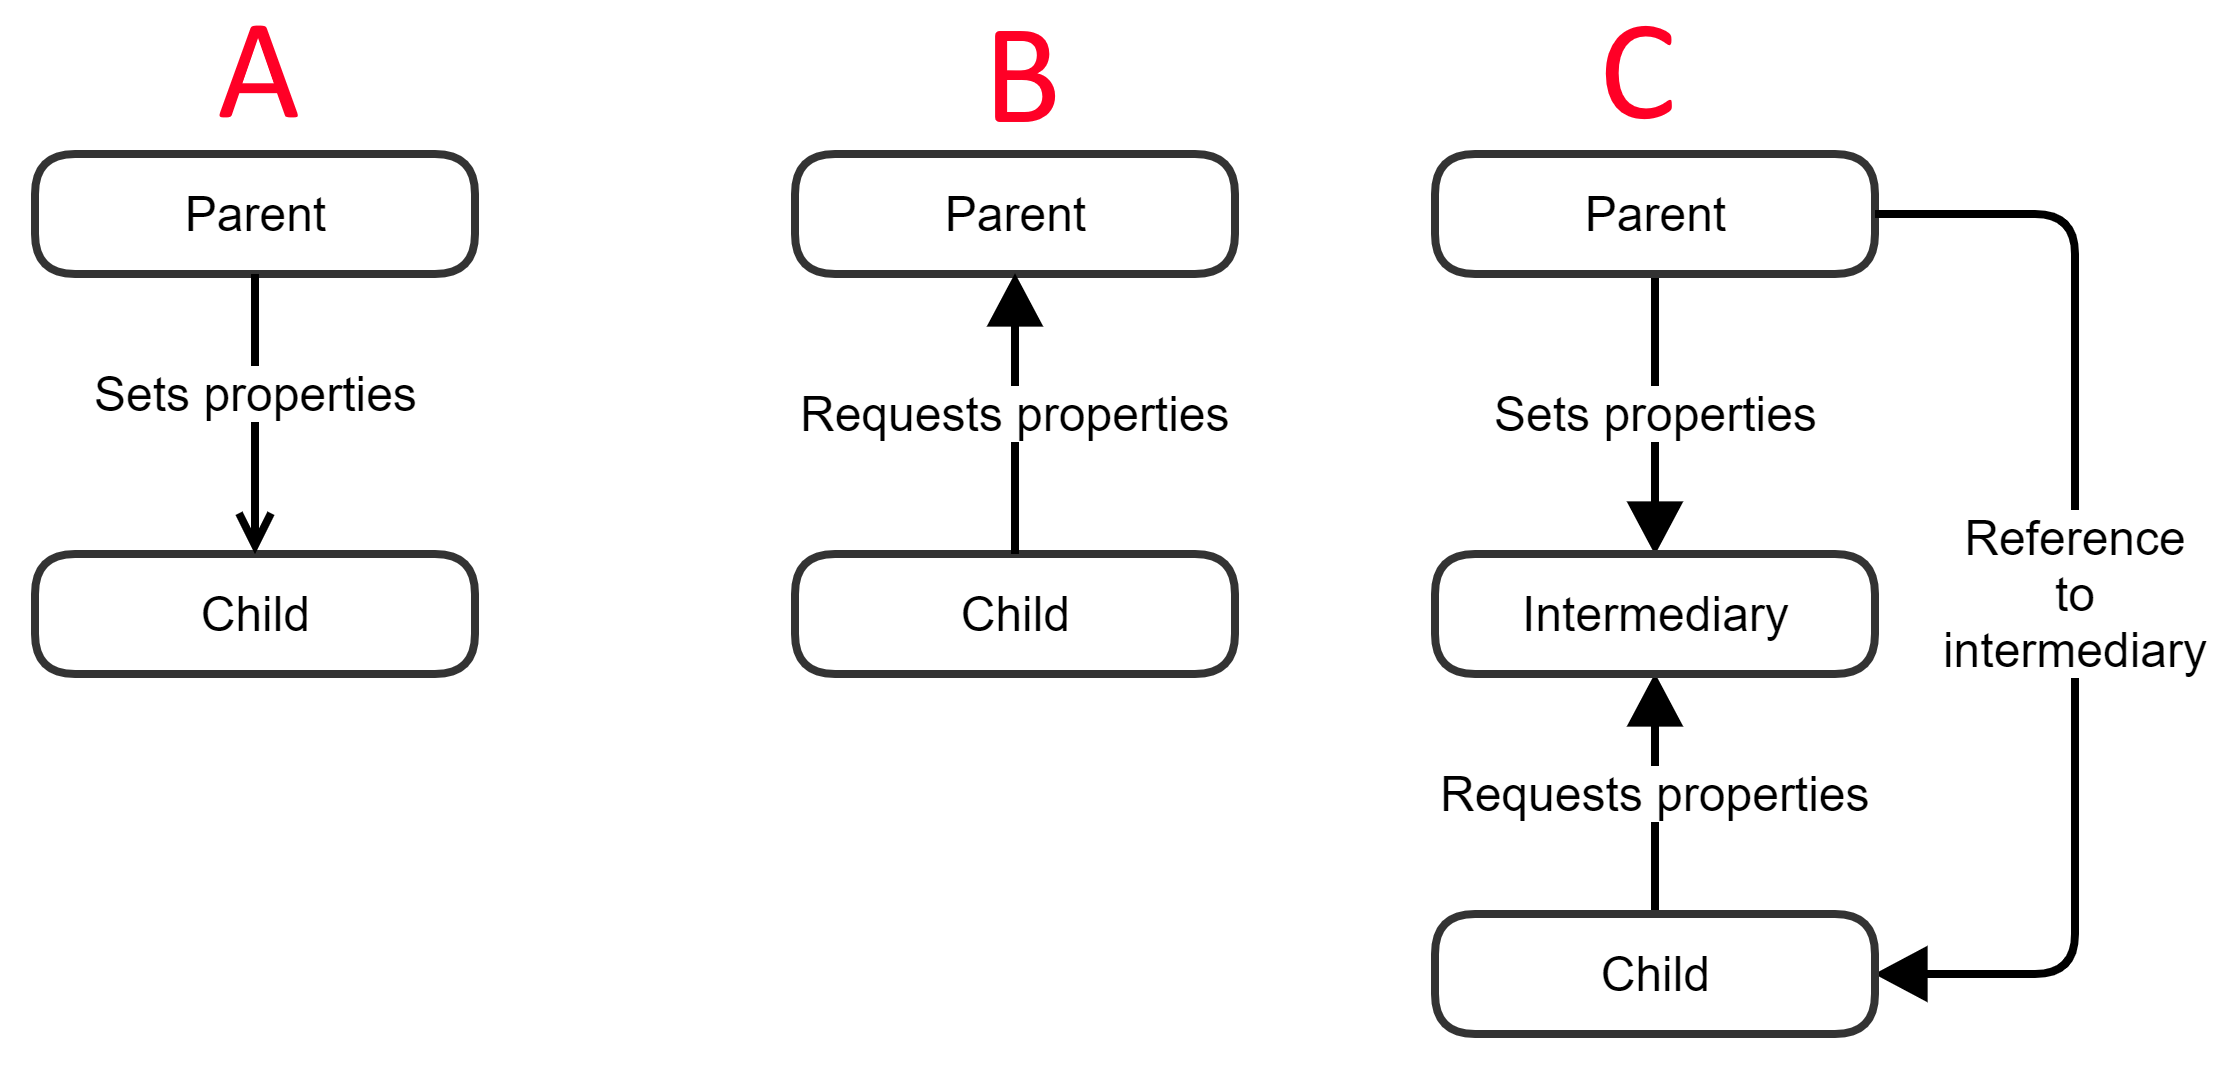
\includegraphics[width=\columnwidth]{figures/case-study/complex-attributes-methods.png}
    \caption{Categories into which approaches to passing complex attributes can be grouped}
    \label{fig:case-study:complex-attributes-methods}
    \centering
  \end{figure}

  \begin{itemize}
    \item \emph{Parent \(\rightarrow\) child (marked A in Figure~\ref{fig:case-study:complex-attributes-methods}):} The parent node gets a reference to the child during the rendering process. Then the parent sets the properties on the child.
    \item \emph{Child \(\rightarrow\) parent (marked B in Figure~\ref{fig:case-study:complex-attributes-methods}):} The child gets a reference to the parent during the rendering process. It then requests its properties from the parent.
    \item \emph{Parent \(\rightarrow\) intermediary \(\rightarrow\) child, Child \(\rightarrow\) intermediary \(\rightarrow\) parent (marked C in Figure~\ref{fig:case-study:complex-attributes-methods}):} An intermediary takes the properties from the parent. The parent then provides the child with some way to find the intermediary, after which the child can get the properties from the intermediary upon rendering.
  \end{itemize}

  The first approach would be the easiest, but this approach is not always feasible. Many JS frameworks do not provide such low-level access to the to-be-rendered component. Instead, they often provide callbacks with a reference to the element after it has been connected to the DOM\@. Since the properties of our components need to be defined before they have even been rendered, this approach does not work for us.

  The second approach presents similar problems. While in some JS frameworks, it is possible to get a reference to the parent component, JS frameworks that use a virtual DOM such as ReactJS and Vue~\footurl{https://vuejs.org/} do not have a real parent component instance. Instead, the parent is just an abstract concept.

  This leaves us with the last approach—the creation of an intermediary object which holds the properties. The child is then given some way to get a reference to the intermediary (bypassing the problem of the second approach), after which it can get the to-be-applied properties from the intermediary. As long as we make sure the child has a way to find the intermediary access before it has been rendered to the DOM, we are able to fulfill the requirement of defining all properties before the first render.
}{
  Our implementation consists of several steps. We start by creating a class which we will call \emph{Intermediary}. This class has an instance manager attached to it, which we will call the \emph{IntermediaryManager}. Our JS framework wrapper code will be wrapping around the basic CC UI library. Since the CC UI library does not export the IntermediaryManager, we are unable to get a reference to it from our wrapper (aka the parent). In order to still get a reference to it, we want to store it globally. Because storing such properties on the \code{window} object can result in collisions and is unreliable, we will be storing it as a property of the defined Web Components. This means that we are able to access the \code{IntermediaryManager} property on the  \code{customElements.get('cow-checkbox')} object and get a reference to the IntermediaryManager from both the parent side and the child side.

  Now that we have taken care of this issue, we are able to start using it. We make the parent create an instance of an Intermediary. This Intermediary gets a simple string ID\@. We are then able to look up the ID in the IntermediaryManager and get the corresponding Intermediary. This ID is passed to the child, allowing it to look up this Intermediary.

  For passing the actual values, we make use of references. For each of the parent's properties, we pass the value to the Intermediary. The Intermediary then generates a unique string representing that value. If the Intermediary already knows the value, the same string is returned. Internally it maps this string to the value. We then pass this string to the child instead of passing the original complex value (which would not work). The child then receives the value and resolves it back to a complex value by consulting the Intermediary. Through this process, the child component is able to receive complex values from its parent through simple HTML string attributes.
}

\section{Angular Issues}
In this section, we describe any Angular related issues we faced. These are issues that were specific to Angular and are unlikely to be faced in similar projects when a different JS framework is being targeted.

\subsection{A1: ng-deep}\label{sec:case-study:ng-deep}
\problemSolution{
  Angular provides the \code{ng-deep} CSS selectors~\footurl{https://angular.io/guide/component-styles\#deprecated-deep--and-ng-deep}. Where regular CSS selectors stop at the ShadowDom boundary, meaning that a component will never be able to have a selector apply to the DOM of another component, the ng-deep selector does allow for this. This selector is deprecated but still in use in the 30MHz codebase. It is a CSS selector that is implemented in JavaScript by Angular that does not work outside of Angular environments (including the Web Components environment). As such, we need to remove it.
}{
  The fix for this issue was fairly simple. Any instance of ng-deep had to be removed. While there has been some talk around browser support for a similar deep selector~\footurl{https://drafts.csswg.org/css-scoping/}, with both \code{::shadow} and \code{/deep/} making it into Chrome, they have since both been removed~\footurl{https://developers.google.com/web/updates/2017/10/remove-shadow-piercing}. As such, we had to come up with a workaround. Since the only way to effectively communicate from a component to child components is properties, we changed the code to use properties instead. An example of this change can be seen in Listing~\ref{lst:case-study:ng-deep-before} and Listing~\ref{lst:case-study:ng-deep-after}.
}

\begin{lstlisting}[language={JavaScript},caption={A component before the ng-deep change},label={lst:case-study:ng-deep-before}]
// parent-component.html
<child-component></child-component>

// parent-component.css
::ng-deep div {
  color: red;
}

// child-component.ts
@Component({
  ...
})
class ChildComponent {
  ...
}
\end{lstlisting}

\begin{lstlisting}[language={JavaScript},caption={A component after the ng-deep change},label={lst:case-study:ng-deep-after}]
// parent-component.html
<child-component red></child-component>

// child-component.ts
@Component({
  ...
})
class ChildComponent {
  @Input() red: boolean;

  constructor(private _elementRef: ElementRef) {
    if (this.red) {
      _elementRef.nativeElement.classList.add('red');
    }
  }
}

// child-component.css
:host[red] {
  color: red;
}

\end{lstlisting}

\subsection{A2: createCustomElement}\label{sec:case-study:create-custom-element}
\problemSolution{
  The main export of the Angular Elements library is the \code{createCustomElement} function~\footurl{https://angular.io/api/elements/createCustomElement}. This function takes an Angular component and turns it into a Web Component. It does this by extending an \code{HTMLElement} base class and applying all Angular component features on top of it. However, this function does not offer the ability to change the base class from an \code{HTMLElement} into anything else. As mentioned before, the 30MHz dashboard makes use of some elements that extend native elements. For example, the 30MHz input field extends the default HTML input field and only adds styling, preserving any built-in accessibility features provided by the browser. When migrating this Angular component to a Web Component, we also wish to preserve these same features. This can be done by extending built-in HTML elements~\footurl{https://developer.mozilla.org/en-US/docs/Web/Web_Components/Using_custom_elements}. The \code{createCustomElement} function does not provide this option, causing us to be unable to create such an element. There is an open feature request for this option at the time of writing of this paper~\footurl{https://github.com/angular/angular/issues/19108}.
}{
  We have no choice but to implement this option ourselves. This means we have to copy the entire source code of the \code{createCustomElement} function, along with many of its dependencies, since very few of them are exported. After this, we change the function to allow us to pass such an option. It should be noted that this does introduce additional difficulties with upgrading Angular Elements. Instead of upgrading the package itself, the copied source code will have to be replaced with the new source code. On the other hand, the referenced issue might be fixed, after which the process of copying source code is no longer necessary.
}

\subsection{A3: EventEmitters}\label{sec:case-study:eventemitters}
\problemSolution{
  Angular implements \code{EventEmitters}~\footurl{https://angular.io/api/core/EventEmitter}. These are classes that are able to emit events, as well as being able to be listened to. When the \code{emit} function is called, the passed value is sent directly to those functions that added an event listener to it. Note that this behavior is different from regular event emitters, which emit a \code{CustomEvent}, which contains the actual value in the \code{detail} property. A lot of our Angular code relies on the value being directly emitted and it not being wrapped in a CustomEvent.

  When a component is migrated to a Web Component, however, this emitted value is wrapped in a CustomEvent. Since the Angular code relies on this value being directly emitted, errors occur. In order to get around this issue, we need to make sure that internal code that listens to such EventEmitters receives the value itself, while external code (such as a 3rd party listening to a Web Component) receives the value wrapped in a CustomEvent.
}{
  We run a script that iterates over the source files, looking for any location where an event listener is being added to such an EventEmitter. Once we find one, we wrap the callback in an unwrapping function that strips away the CustomEvent and returns just the \code{code} value. An example of this change can be seen in Listing~\ref{lst:case-study:event-handler-change}.
}

\begin{lstlisting}[language={JavaScript},caption={A change made to an event listener. The definition of \code{unwrapEvent} can be seen in Listing~\ref{lst:case-study:event-handler-unwrap-event}},label={lst:case-study:event-handler-change}]
// before
(valueChanged)="myHandler($event)"

// after
(valueChanged)="myHandler(unwrapEvent($event))"
\end{lstlisting}

\begin{lstlisting}[language={JavaScript},caption={The \code{unwrapEvent} function},label={lst:case-study:event-handler-unwrap-event}]
function unwrapEvent(event) {
  if (event instanceof CustomEvent) {
    return event.detail;
  }
  return event;
}
\end{lstlisting}

\subsection{A4: Hierarchical Injectors}\label{sec:case-study:hierarchical-injectors}
\problemSolution{
  Angular makes use of a feature called \emph{Dependency Injection}~\footurl{https://angular.io/guide/dependency-injection}. This allows a parent module to provide its children with an instance of a particular dependency class. This class instance is shared among the module and its children. Generally, only modules provide their children with dependencies, where modules are simply collections of components that serve some common purpose. This dependency injection feature can also be leveraged to have a given component provide its own instance of a class only to its direct children. This means that every instance of that component gets its own separate instance of the dependency, which it then shares with its children, and not one that is shared across all components in the module. This is called \emph{Hierarchical Dependency Injection}\footurl{https://angular.io/guide/hierarchical-dependency-injection} and it is a feature that is utilized by 30MHz in some areas.

  Angular Elements does not support this feature intentionally~\footurl{https://github.com/angular/angular/issues/24824\#issuecomment-404399564}. Instead, it only supports the use case where modules provide their components with dependencies. The reason for this is that every component migrated with Angular Elements is mounted to the DOM as its own root. It does not have a concept of a parent component and is unable to look up the injector of its parent. While the pattern of Hierarchical Dependency Injection is not recommended for use with Angular Elements~\footurl{https://github.com/angular/angular/issues/24824\#issuecomment-404399564}, it is still a pattern used by 30MHz, and as such, we need to support it in order for the CC UI library to work.
}{
  Our goal in fixing this problem is to have a component injector inherit from its parent injector, which will facilitate Hierarchical Dependency Injection. To do this, we need to find the parent when the child is being rendered. After this, we can extract its injector, craft a new injector that combines the child and parent injector, and finally supply this new injector to the child. An example of this process can be found on StackBlitz~\footurl{https://stackblitz.com/edit/ngelements-issue-40104?file=src\%2Fapp\%2Fbar\%2Fbar.component.ts}.

  We first need to find the parent. This process is relatively straightforward. When the child is being rendered, we travel up the DOM tree until we find a node with specific properties that only Angular elements have. We then move on to the next stage of finding its injector.

  While the finding of a node's injector is straightforward in development mode since Angular exposes a \code{window.ng.getInjector} function, this process is a lot more complicated in production mode. To find it, we first need to find the component's hidden Angular properties. These can be found under the component's \code{\_\_ngContext\_\_} property. Depending on the environment, this can either be an object containing the \code{tNode} and \code{lView} properties or an array that contains them at a magic offset. The \code{tNode} and \code{lView} are internal representations of a bunch of Angular-specific properties for the component.

  We are unable to access the original injector of the parent component since it is hidden in Angular-internal code. Instead, we need to use the \code{tNode} and \code{lView} to craft a new injector that will do the same thing as the original injector. However, in order to craft this new injector class instance, we need a reference to that same class. While a \code{Injector} class is exported from the Angular package, this is not actually the injector we want. Angular actually has two types of injectors, one of which is the previously mentioned \code{Injector} and the other is the \code{NodeInjector}. This \code{NodeInjector} is only used internally, and it is the injector we want. To get a reference to it, we access the \code{injector} property of a fake component created by a \code{ComponentFactory}. Since the \code{ComponentFactory} is also not exported, we need to get a reference to it through the global injector. We now finally have a reference to the \code{NodeInjector} class, which allows us to re-create the parent's injector.

  We now merge this injector with the child injector. This is a relatively simple process. When a request for an injected value comes in, we first look for it in the child. If the child does not have it, we look at the parent injector.

  We now need to make sure Angular actually uses this injector we just created. To do so, we need to override the component's default element strategy (\code{NgElementStrategy}). This element strategy is a class provided by Angular that manages the connection between the DOM and the underlying Angular component. Since the \code{NgElementStrategy} class is also not exported by Angular, we need to find a reference to it somewhere. To do so, we create a fake component and read its \code{ngElementStrategy} property. We can now extend the class, replace the injector and provide it to the component. A complete code example of this process can be found in Listing~\ref{lst:appendix:hierarchical-injectors}.

  While we attempted to maintain compatibility with the Angular source code by not copying code but by instead getting references to them at runtime, Angular updates might cause the current solution to this problem to break. While the underlying idea for the solution is unlikely to be rendered impossible, the methods we use to achieve it might change, and the code might have to be partially re-written.
}

\subsection{A5: ngOnInit}\label{sec:case-study:ng-on-init}
\problemSolution{
  Angular Elements does intentionally not guarantee the order in which attributes are set on an element (even initial attributes)~\footurl{https://github.com/angular/angular/issues/29050}. This means that attributes can be set on an element both before or after its main init hook (\code{ngOnInit}) is called. An example of this process can be seen in Listing~\ref{lst:case-study:ng-on-init}. While this is not a problem if attributes are only used to handle visual state, they can cause significant problems when used for component configuration. For example, if a component performs a fetch request to the server and takes a \code{URL} property that determines the target URL, it is essential that this property be set before the main hook runs. Quite a few components in the 30MHz codebase have a similar setup. As such, we need to guarantee that a component will always have the complete set of initial properties set before its main hook is called.
}{
  We know that, while the order of attribute setting is not guaranteed, we are guaranteed the fact that they will run sequentially. Since JavaScript is a single-threaded language and all attribute setting calls are synchronous, we know that all attributes will be set once the main thread is free again. For this, we use the global \code{window.requestAnimationFrame} JavaScript function. This function takes a callback and calls it when the main JavaScript thread is free to take on new work. We now firstly replace the component's \code{ngOnInit} function with an empty function, ensuring that when Angular calls it, the component's main hook is not actually run. We then call \code{window.requestAnimationFrame} and pass it the original \code{ngOnInit} function. Now we can guarantee that the \code{ngOnInit} function is called after all attributes have been set.
}

\begin{lstlisting}[language={JavaScript},caption={HTML source code and its Angular Elements equivalent},label={lst:case-study:ng-on-init}]
// HTML source file
<my-element foo="bar" bar="baz" />

// can be transformed into any of the following:
// 1
const element = document.createElement('my-element');
element.setAttribute('foo', 'bar');
element.setAttribute('bar', 'baz');
parent.appendChild(element);

// 2
const element = document.createElement('my-element');
parent.appendChild(element);
element.setAttribute('foo', 'bar');
element.setAttribute('bar', 'baz');

// 3
const element = document.createElement('my-element');
element.setAttribute('foo', 'bar');
parent.appendChild(element);
element.setAttribute('bar', 'baz');
  \end{lstlisting}

\subsection{A6: Casing in attribute names}\label{sec:case-study:casing}
\problemSolution{
  In the process of migrating Angular components to Web Components, Angular Elements maps all input properties from camelCase casing to kebab-case. For example the input property \code{myInputProperty} is set through the \code{my-input-property} HTML attribute. The reason for this change is that HTML attributes are case-insensitive. To HTML \code{myInputProperty} is identical to \code{myinputproperty} and \code{MYINPUTPROPERTY}. This mapping of input properties presents some issues to us. Internal Angular elements still use the camelCase variant to set properties on their child components. Since the Web Component variants do not recognize the camelCase variant of the property anymore, they are ignored.
}{
  We solve this issue by making sure the Web Components also accept the camelCase variant. As HTML is case insensitive, there is no point in checking the casing of the passed attribute. Instead, we convert it to lowercase and compare it against the lowercase version of the original camelCase input property. In the previous example \code{myInputProperty}, \code{myinputproperty}, \code{MYINPUTPROPERTY}, and \code{my-input-property} would all refer to the input property \code{myInputProperty} on the Angular component.
}

\subsection{A7: Angular directives}\label{sec:case-study:directives}
\problemSolution{
  Angular has two types of elements that appear in the DOM\@. The first type is the Component, which looks for a given selector or tag name and replaces the original HTML element. For example an \code{AppRootComponent} with the selector \code{'app-root'} will look for an \code{<app-root>} HTML element and replace it with the Angular component instance. The second type is the Directive. Similarly, this looks for a selector, but instead of replacing the original HTML element, this simply mounts to it and runs its own code on it. An example of this would be a \code{Blink} directive that looks for the \code{'blink'} HTML class. When mounted, it periodically hides and un-hides the component.

  Angular Elements only supports the conversion of Components to Web Components, not the conversion of Directives. Since there are some elements in the 30MHz codebase that use Directives, we need to make sure that these are supported as well.
}{
  While this might sound like a challenging problem since these are entirely different elements, the fix for this issue is surprisingly easy. Under the hood, Angular stores the definition of a Component in the \code{\cmcrv{}cmp} property. This is also the property Angular Elements accesses to do the migration from Angular components to Web Components. Similarly, the definition of Directives is stored in the \code{\cmcrv{}dir} property. By simply copying the value of the \code{\cmcrv{}dir} property to the \code{\cmcrv{}cmp} property, we are able to trick Angular Elements into thinking a directive is a component. Surprisingly, this works, and the directive works perfectly.
}

\subsection{A8: <ng-content>}\label{sec:case-study:ng-content}
\problemSolution{
  Angular uses the \code{<ng-content>} tag for content projection. Content projection is the ability for a component to take a set of children, which it can then place anywhere in its DOM tree. This is effectively the same as the HTML \code{<slot>} tag~\footurl{https://developer.mozilla.org/en-US/docs/Web/HTML/Element/slot}. An example of content projection can be seen in Listing~\ref{lst:case-study:ng-content}. Content projection works fine in most scenarios, but for unknown reasons, it sometimes does not work. The result is that child elements simply do not show up.
}{
  Our solution is once again quite simple; we take advantage of the fact that the \code{<ng-content>} and \code{<slot>} tag do the same thing and append a \code{<slot>} tag to every occurrence of an \code{<ng-content>} tag in the source code. This ensures that when the \code{<ng-content>} tag does not work, the \code{<slot>} tag takes over instead. Since the browser only allows a given child element to be projected into one spot (\ie{} multiple \code{<slot>} tags do not result in multiple copies of the child element), this approach will not cause any problems in cases where \code{<ng-content>} does work.
}


\begin{lstlisting}[language={HTML},caption={HTML source code and its Angular Elements equivalent},label={lst:case-study:ng-content}]
// parent-component.html
<child-component>
  <span id="my-span"></span>
</child-component>

// child-component.html
<div id="my-root">
  <ng-content></ng-content>
</div>

// Effective DOM tree
<parent-component>
  <child-component>
    <div id="my-root">
      <span id="my-span"></span>
    </div>
  </child-component>
</parent-component>
  \end{lstlisting}

\subsection{A9: Angular Attribute Order}\label{sec:case-study:attribute-order}
\problemSolution{
  As previously described in Section~\ref{sec:case-study:ng-on-init}, the order in which Angular attributes are set is unknown. While we have fixed this issue for our Web Components in this section, this same issue presents itself again in the writing of an Angular wrapper. This time the problem is that components will be rendered before they have all of their input properties set. This leads to the apparent issue where the wrong contents are rendered.

  Another problem stems from our approach in Section~\ref{sec:case-study:complex-attributes}. We pass a unique ID to the child that is used to find the intermediary. When the child now receives an attribute that starts with the special reference prefix, it looks up the given reference by finding the intermediary and reading the attribute value. However, if the child receives such an attribute before having received the unique ID of the intermediary, it is unable to resolve the value. Since the order in which Angular attributes are passed is unknown, this situation arises very often.
}{
  We get around these issues by handling the appending to the DOM ourselves. Instead of having our Angular wrapper render the actual Web Components, we instead have them render a \emph{Renderer} component. This component is then passed the tag name of the Web Component. We are now able to precisely control when a component is appended to the DOM, as well as which attributes it gets and in what order. Since the \emph{Renderer} takes the place of the Web Component, it now receives all attributes. We wait until it has received the very last attribute before we decide to create the child component. After creating it, we apply all attributes the \emph{Renderer} has received to the child, after which we append it to the DOM\@. Since this process allows us such fine-grained control over the rendering cycle, we are able to render the Web Component without any issues.
}

\subsection{A10: Bundling Angular Imports}\label{sec:case-study:bundling-imports}
\problemSolution{
  Angular provides a few ways to build projects. Two of which are in use by us. The first option is to build a project as an application. This bundles everything into a combination of browser-specific bundles. These bundles can then smoothly be loaded by including them in the browser. This is the option we use for the Web Component library. The second option is to build a project as a library. Building a project as a library preserves all typing information and allows it to be used by another Angular project. Since we are building an Angular project, this is the option we need if we want to be able to provide typings to developers who use our Angular wrapper.

  However, we run into an issue after building. 30MHz uses the Font Awesome Pro~\footurl{https://fontawesome.com/pro} package for its icons. This is a licensed package that can only be downloaded when a valid key is presented. Since some of these icons are also used in the CC UI library, it needs to be bundled into the library to be able to work. Angular refuses to do this. They recommend using \code{peerDependencies}~\footurl{https://github.com/ng-packagr/ng-packagr/blob/v10.1.0/docs/dependencies.md} instead. While their reasoning for this is valid, it does not apply in our case. Since third-party developers are unable to install the Font Awesome Pro package without a license, they would run into an error when installing the package. Previously, Angular had the \code{embed} option, which allowed for the embedding of a given set of JS packages. This was eventually replaced with \code{bundledDependencies}~\footurl{https://github.com/ng-packagr/ng-packagr/issues/1106}, and a little while later, it was deprecated~\footurl{https://github.com/ng-packagr/ng-packagr/commit/0c52486}. This leaves us with no native option to bundle our dependency.
}{
  We fix this issue by programmatically changing the build artifacts Angular outputs. There are three types of build formats, the \code{FESM2015} (or flattened \code{ESM2015}), \code{ESM2015}, and \code{umd} formats. Bundling the Font Awesome Pro source code is fairly trivial for the \code{FESM2015} and \code{umd} formats since they are both single files. The \code{ESM2015} format is a bit different. It consists of a folder that is essentially a clone of the source code, with every TypeScript source file being replaced with a compiled JavaScript version and a \code{.summary.json} file. This \code{.summary.json} file functions similar to a \code{.d.ts} file, in that it provides type information of the file. In fixing our issue, we want to preserve this same folder structure. This means that we can not simply pass the entry point to a bundler and be done. On the other hand, we are also not able to feed every individual JavaScript file to the bundler. This would result in every separate file including its own copy of the Font Awesome Pro library, leading to a significant bundle size. Instead, we create a central folder in the \code{ESM2015} folder in which we store the Font Awesome Pro JavaScript bundle. This folder functions the same as a \ver{node\_modules} folder. We now replace every reference in the source files to point to this central location instead.
}

\problemSolution{
  We now run into another problem. When the library that was just built is used in an Angular project, the Angular compiler scans over all of its \code{.summary.json} files to build an AST with type information. It then finds the values that are exported, looks up their type values in the AST, and exports those that correspond to them. In performing this AST building process, the Angular compiler scans our included Font Awesome Pro folder for \code{.summary.json} files in order to extract definitions. Since those do not exist, an error is thrown.
}{
  The obvious approach to this problem is the following. We generate and bundle along the \code{.summary.json} files. This will provide Angular with the definitions it needs. The downside to this is that Angular will recursively perform this AST building process, meaning that it will first scan Font Awesome Pro, then its dependencies and their dependencies. All of these files would need to be included in the bundle simply to ensure the Angular compiler does not throw an error.

  Instead, the solution is to simply remove any reference to our bundled Font Awesome Pro library from the \code{.summary.json} files. Now that there is no longer a reference, the Angular compiler will simply skip over it. Since the Font Awesome Pro library is not exported, the Angular compiler never has to export any of its type information, meaning it does not actually need this data.
}

\subsection{A11: Angular Ivy}\label{sec:case-study:ivy}
\problemSolution{
  Angular has released a new version of its compiler called Ivy~\footurl{https://angular.io/guide/ivy}. This Ivy compiler is set to replace the previous View Engine compiler. Angular does not allow the use of Ivy for projects built as libraries for now~\footurl{https://angular.io/guide/ivy\#maintaining-library-compatibility} both because of compatibility reasons and because Ivy is not seen as stable enough as of the writing of this paper. This forces us to use the View Engine compiler instead. This compiler contains several bugs, one of which is causing the build to fail entirely in our case~\footurl{https://github.com/angular/angular/issues/25424}. This bug is marked as \ver{Fixed by Ivy}; however, we are unable to use Ivy.
}{
  The only other fix to this issue seems to be the disabling of AOT (or ahead-of-time compilation~\footurl{https://github.com/angular/angular/issues/25424\#issuecomment-465643237} and it is the solution we have applied to this problem. Unfortunately, the disabling of AOT introduces significant overhead during the loading of the built library, an issue that we have not been able to fix. As will be mentioned in the results section, this increases the load time of the Angular wrapper to an unacceptable level. We have chosen to still disable AOT compilation as it shifted the issue from a blocking one (the inability to compile the code at all) to a performance issue.
}

\section{Optimizations}
After finishing the CC UI library, we started looking for performance optimization opportunities. By looking through the Chrome profiler trace, we were able to find some easy performance improvements. These are discussed in detail below.

\subsection{O1: Reduce time searching for CSS}\label{sec:case-study:searching-for-css}
We provide developers with a CSS file they should include in their final \code{index.html} file. This file contains the styles required to make the CC UI library work. We refer to this CSS file as the CC CSS file from now on.

As mentioned in Section~\ref{sec:case-study:global-css}, we find the CC CSS file on the page and copy it into every component instance. Since there can be many more stylesheets than just the CC CSS file, we need to scan every stylesheet and check whether it is the one. This searching process consists of the following steps.

\begin{itemize}
  \item Get a list of all stylesheets on the page, this includes both \code{<style>} tags and \code{<link rel="stylesheet">} tags.
  \item Iterate through every stylesheet.
  \item Iterate through every rule.
  \item Compare the current rule with a specific marker value that signifies the CC CSS file. If it matches, move on to the next step
  \item Add this stylesheet to the list of CC CSS files and move on to the next stylesheet.
\end{itemize}

While we did implement some caching, making sure this process only runs a single time, this process still has a significant performance impact. This performance impact scales linearly with the size of the stylesheet, meaning that a stylesheet with more rules takes longer to scan. It takes about 16ms to scan through a stylesheet of 1667 lines in order to find the marker rule on the machine mentioned in Section~\ref{sec:experimental-setup:machine-specs}. In addition to scaling with the size of the stylesheet, this number also scales with the number of stylesheets. Since it iterates through every available stylesheet, including a big stylesheet will vastly increase loading times. A rough formula for this performance impact in milliseconds can be found in the equation below, with \(SS\) being a set of all stylesheets and \(LOC\) being the number of lines of code.

\[ t_{ms} = \sum_{i \in SS} \frac{i_{LOC}}{100} \]

We improve this process in two ways. The first step is to stop scanning after we find the marker simply. Instead of looking for other CC CSS files, we simply stop and return early. Since we know that there is only a single CC CSS file that applies to our Web Components, we can make this change. The performance impact of this change is hard to express in a single number since it largely depends on the stylesheets on the page, but this performance improvement saves about 1ms per 100 rules in stylesheets that are not the CC CSS file.

The second step is to ask the developers to help us in this process. We ask them to add a simple \code{cow} attribute to the \code{<style>} or \code{<link rel="stylesheet">} tag that contains the CC CSS file. Since the developer knows which file contains our supplied CSS file, they should easily add this attribute. At runtime, we check whether any stylesheet tags have a \code{cow} attribute. If there are, we can skip the entire process of finding the CC CSS file. Since this process was performed as the first component was rendered, this change saves about 16ms on the first component's render time.

\subsection{O2: Move CSS searching to initial load}\label{sec:case-study:css-initial-load}
While the above fixes provide excellent performance improvements, it may very well be possible that the developer does not add the \code{cow} tag, preventing our performance improvements from applying. The performance impact of the CSS search is still considerable, and the fact that it is run during the rendering of the first component significantly increases its render time. Since these render times tend to be around 16ms by themselves, a 16ms increase is enormous.

We remove this performance impact from the first render by moving it to the moment the CC UI library is initialized. To ensure we do not add any time to the initial load, we wait until the browser is idle by calling \code{window.requestIdleCallback}. This ensures that the process of finding CSS is performed while the browser is idle instead of it blocking an important operation such as component rendering.

\section{JS Framework Wrappers}\label{sec:js-framework-wrappers}
To improve the developer experience, we wrote JS framework wrappers for a total of three JS frameworks, namely ReactJS, Svelte and Angular. In ReactJS, complex attributes for Web Components do not work natively. A wrapper for ReactJS was required in order to get the CC UI library to work in the first place. Since ReactJS provides good tooling when it comes to components and their properties, we felt it was a good idea to make use of this by providing typings for the CC UI library ReactJS wrapper. The second JS framework is Svelte. While Svelte works perfectly with Web Components out of the box, we created a wrapper to provide typings for the developers similar to ReactJS. The last JS framework is Angular itself. Angular also provides tooling, including built-in checking of component properties, which we felt we had to provide.

We also looked at different JS frameworks but found most of them to have little to no tooling for HTML elements. The UI libraries we looked at were Vue (v2 and v3)~\footurl{https://vuejs.org/}, Polymer~\footurl{https://www.polymer-project.org/}, lit-element~\footurl{https://lit-element.polymer-project.org/}, and wc-lib~\footurl{https://www.npmjs.com/package/wc-lib}.

In creating these wrappers, we started off by extracting the required component and type data from the components' source files. For example, the list of input properties, as well as their types and descriptions, need to be known. Similarly, all events emitted by the component, their types, and descriptions also need to be known. Finally, we also need to collect some metadata on the component itself, such as the name, tag name, and whether it has child elements. We extracted all this data by using the \emph{typescript} package~\footurl{https://www.npmjs.com/package/typescript}. This package allows for the parsing of TypeScript and JavaScript code. This code is turned into an abstract syntax tree (AST) with added type information, after which we are able to iterate through it. We extract all this data and turn it into a common format to be re-used by the various scripts that generate JS framework wrappers.

After collecting this data, we are able to generate the various JS frameworks. Generating wrappers was a reasonably smooth process for most JS frameworks. It consisted of iterating through the extracted component data and generating source files written in the language of the JS framework. These source files were then fed into a bundler and bundled into the wrappers. This process went smoothly for both the ReactJS and Svelte wrapper. During the process of creating an Angular wrapper, on the other hand, we faced a few challenges. These challenges are described in detail below.

